\section{Descripción TAMA}

En \cite{KOU2008} se introdujo un método novedoso para el análisis del \entrainment acústico/prosódico. Esta técnica consiste, a grandes rasgos, en armar dos series de tiempo para cada uno de los interlocutores y luego utilizar herramientes de análisis sobre las series construídas. Una serie de tiempo, en términos coloquiales, es una colección cronológica de observaciones, como pueden ser los valores de las acciones de una empresa a lo largo del tiempo, o la cantidad de lluvia medida en \emph{ml} para cada mes de cierto año. En el apéndice \ref{sec:time_series} describimos más en detalle los conceptos básicos sobre series de tiempo.

Un problema que resuelve esta técnica es el del alineamiento: si intentásemos comparar cada segmento del habla (utterance) con otros, ¿cómo los alineamos? Una posibilidad sería uno a uno, aunque ésto es muy simplista y poco representativo de la realidad. Al introducir el concepto de series de tiempo, podemos olvidarnos de los segmentos del habla y simplemente utilizar estas construcciones.

Para construir la serie de tiempo de cada interlocutor debemos, en primer lugar, dividir el diálogo en ventanas solapadas de igual tamaño. A la diferencia entre ventana y ventana llamaremos \emph{frame step}, y al tamaño de ventana \emph{frame length}. Consideraremos sólo los segmentos de habla que se encuentren dentro de cada ventana; aquellos segumentos que atraviesen los límites de las ventanas son cortados para que se mantengan dentro de éste. En la figura \ref{tama} se ilustra el proceso.

Como producto de ésto, nuestro corpus queda dividido en una sucesión ventanas solapadas. En el trabajo original, se usa un step de 10 segundos, y un tamaño de ventana de 20 segundos. Ésto da como resultado un solapamiento del 50\%. En la sección \ref{sec:window_selection}, describimos la elección del tamaño de ventana que hicimos en base al corpus que utilizamos.

\begin{figure}
\centering
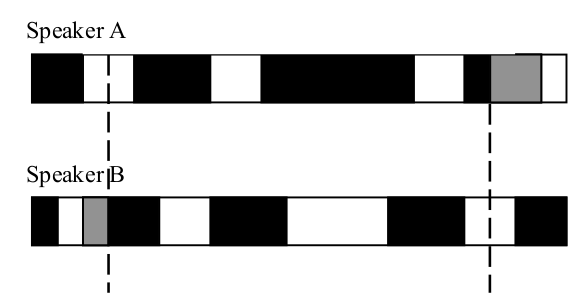
\includegraphics[width=10cm]{images/tama.png}
\caption{Gráfico de la separación del diálogo en ventanas}
\label{tama}
\end{figure}

Una vez que la conversación se ha partido en ventanas mediante el proceso descripto, se calculan los valores de la serie de tiempo para cada interlocutores de cada una de ellas. Ésto se hace mediante el siguiente cálculo:

\begin{equation}
    \mu = \sum\limits_{i=1}^N f_i d_i^\prime \label{eq:tama_mean}\\
\end{equation}

donde $i$ itera sobre las elocuciones dentro del \emph{frame}, $d_i^\prime$ es la duración relativa del segmento (respecto del tiempo total hablado) y $f_i$ es el valor de la \emph{feature} que estamos midiendo. $d_i^\prime$ se calcula con la fórmula

\begin{equation}
dr_i = \frac{d_i}{\sum\limits_{i=1}^N d_i}
\end{equation}

donde $d_i$ es la longitud en segundos de los segmentos del habla en el frame.

Como se ve en \ref{eq:tama_mean}, el valor que calculamos es una media ponderada del valor de la feature por la duración de las locuciones. Así, por ejemplo, al calcular una serie de tiempo sobre la intensidad, la contribución de interjecciones (\emph{ah!} por ejemplo), que suelen tener altos valores \emph{volumen}, estará disminuída por sus breves duraciones.

Una vez obtenidas, dado un feature acústico/prosódico y una conversación, dos series de tiempo mediante el cálculo ventana a ventana de \ref{eq:tama_mean}, necesitamos efectuar algún tipo de análisis sobre éstas para obtener una medida del \entrainment.

\nota{Mejorar el dibujo éste y agregarle una descripción}
